\documentclass[journal=jcisd8,manuscript=article]{achemso}
\usepackage{graphicx}
\usepackage[table]{xcolor}
\usepackage{verbatim}
\usepackage[subrefformat=parens]{subcaption}
\usepackage[version=3]{mhchem} % Formula subscripts using \ce{}

\author{Andrew McNutt}
\author{Paul Francoeur}
\affiliation[University of Pittsburgh]
{Department of Computational and Systems Biology, University of Pittsburgh, Pittsburgh, PA}
\author{Rishal Aggarwal}
\affiliation[International Institute of Information Technology Hyderabad]
{Center for Computational Natural Sciences and Bioinformatics, International Institute of Information Technology, Hyderabad 500 032, India}
\author{Tomohide Masuda}
\affiliation[University of Pittsburgh]
{Department of Computational and Systems Biology, University of Pittsburgh, Pittsburgh, PA}
\author{Rocco Meli}
\affiliation[Oxford]{Oxford}
\author{Matthew Ragoza}
\author{Jocelyn Sunseri}
\author{David Ryan Koes}
\email{dkoes@pitt.edu}
\affiliation[University of Pittsburgh]
{Department of Computational and Systems Biology, University of Pittsburgh, Pittsburgh, PA}

\title{Supporting Information:\\GNINA 1.0: Molecular docking with deep learning}
\renewcommand{\thetable}{S\arabic{table}}  
\renewcommand{\thefigure}{S\arabic{figure}}
\begin{document}
\begin{figure}
    \centering
    \includegraphics{}
    \caption{Caption}
    \label{fig:my_label}
\end{figure}

\begin{table}[]
    \centering
    \begin{tabular}{|c|c|c|c|c|c|}
       \hline Iteration \# &\begin{tabular}{c}Model\\ Selected\end{tabular}&\begin{tabular}{c}Redocking\\ Performance\end{tabular}&\begin{tabular}{c}Redocking\\Ranking\end{tabular}&\begin{tabular}{c} Crossdocking\\Performance\end{tabular}&\begin{tabular}{c}Crossdocking\\Ranking\end{tabular}\\ \hline
        0 & Crossdock Dense 4 & 37.8 & 5 & 67.7 & 1 \\ \hline
        1 & General Default2018 3 & 70.4 & 6 & 39.8 & 2 \\ \hline
        2 & Crossdock Dense 3 & 71.2 & 7 & 40.4 & 2 \\ \hline
        3 & Crossdock Default2018 0 & 71.7 & 7 & 40.6 & 2 \\ \hline
        4 & Redock Default2018 2 & 72.2 & 1 & 40.1 & ? \\ \hline
    \end{tabular}
    \caption{Optimal Model Selection}
    \label{tab:OptimalModelSelection}
\end{table}

\begin{figure}    
        \begin{subfigure}[b]{0.48\textwidth}    
		\centering
		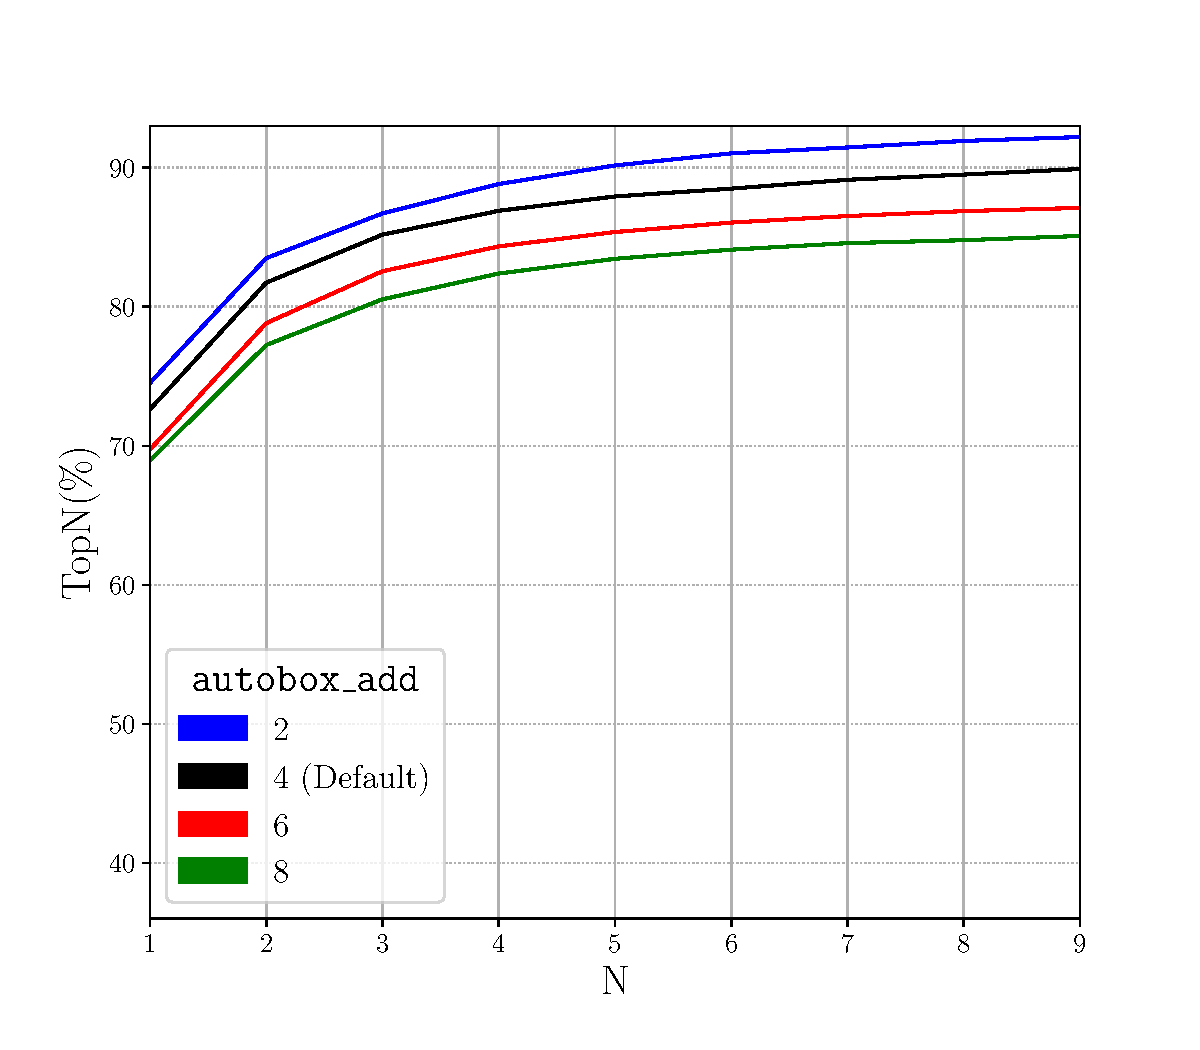
\includegraphics[width=\textwidth]{figures/redocking/sweep_autobox_add_line.pdf}
		\caption{Redocking}
		\label{fig:AutoboxAddRedock}
        \end{subfigure}    
        \begin{subfigure}[b]{0.48\textwidth}    
		\centering
		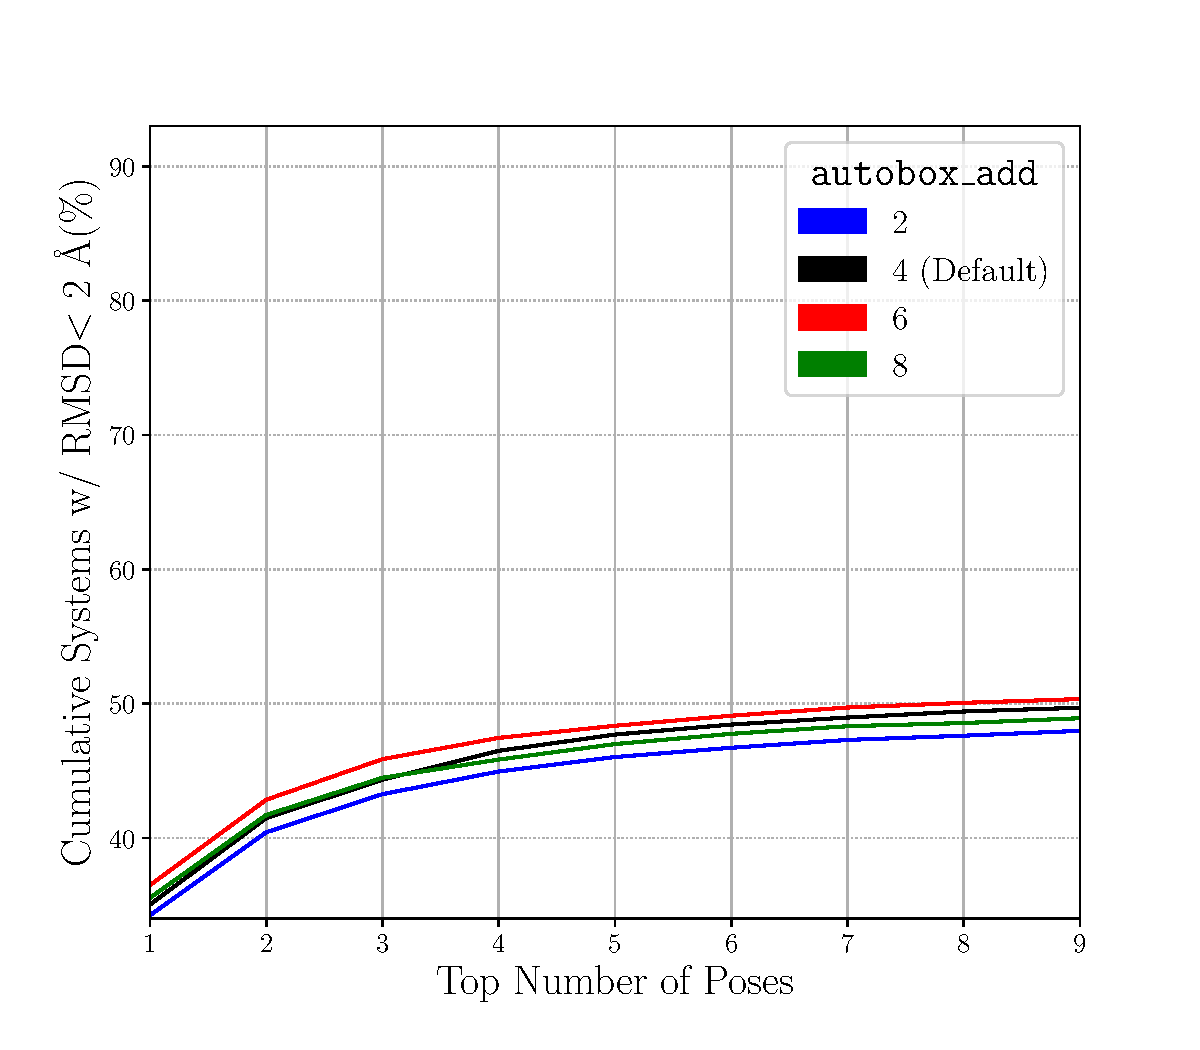
\includegraphics[width=\textwidth]{figures/crossdocking/sweep_autobox_add_line.pdf}
		\caption{Crossdocking}
		\label{fig:AutoboxAddCrossdock}
        \end{subfigure}    
	\caption{Evaluating the affect on docking performance when the value of Autobox Add is changed (move to supplement)}
	\label{fig:AutoboxAdd}
\end{figure}  
\end{document}
